%\documentclass{beamer}
\documentclass[handout]{beamer}

\usepackage[latin1]{inputenc}
\usepackage{pifont}

\usecolortheme{albatross}

\mode<presentation>
{ 
    \usetheme{boxes} 
}


\title{Introduction to the semantic web \\ 
or \\
An overview of tomorrow's web\ldots}
\author{
Pascal Mainini\\
\texttt{pascal <at> impressionet <dot> ch}\\
\texttt{gurke <at> netlabs <dot> org}\\
}
\date{2009-06-06}

\AtBeginSection[]
{
    \begin{frame}<beamer> 
        \frametitle{Outline}
        \tableofcontents[currentsection]
    \end{frame}
}

\begin{document}

    \begin{frame}
        \titlepage
    \end{frame}

    \section{Introduction}

        \begin{frame}
            \frametitle{About me}

            \begin{itemize}
                \item I'm Pascal Mainini
                \pause
                \item Open minded, critical hacker
                \pause
                \item Started with computers almost 20 years ago, working professionally since nearly 10 years
                \pause
                \item Currently working as a network and security specialist
                \pause
                \item \textit{Note: I don't like beeing photographed or recorded otherwise, thanks!}
            \end{itemize}
        \end{frame}

        \begin{frame}
            \frametitle{About this speech}

            This speech will
            \vskip 0.7cm
            \pause

            \begin{itemize}
                \item Give an idea of what the semantic web is about
                \pause
                \item Give an overview of underlying technologies
                \pause
                \item Serve as a starting point for further explorations of the semantic web
            \end{itemize}
        \end{frame}

        \begin{frame}
            \frametitle{About this speech}

            This speech will \textbf{NOT}
            \vskip 0.7cm
            \pause

            \begin{itemize}
                \item Provide an exact mathematical background (I'm too lame for that...)
                \pause
                \item Give an in-depth tutorial of the technologies used (URIs, XML, RDF...)
                \pause
                \item Allow you to start working with semweb-technologies without investing any further work
            \end{itemize}
            \vskip 0.7cm
            \pause
            \textbf{Note: If you have questions - ask them right away...!}
        \end{frame}

        \begin{frame}
            \frametitle{About this speech}

            This speech and additional material is licensed under a ``Attribution-Noncommercial-Share Alike 3.0 Unported'' license:
            \vskip 0.4cm

            \texttt{http://creativecommons.org/licenses/by-nc-sa/3.0/}
            \vskip 0.7cm

            The slides and additional material can (soon) be found at:
            \vskip 0.4cm

            \texttt{http://impressionet.ch/semwebspeech3}
            \vskip 2cm

            \begin{center}
                
\includegraphics[scale=0.5]{somerights}
            \end{center}
        \end{frame}

    \section{The idea behind the semantic web}

        \begin{frame}
            \frametitle{Problems of the current web}

            \begin{itemize}
                \item A gigantic bunch of information, a large diversity of formats
                \pause
                \item This information is stored in a form understandable for humans (which is great!)
                \pause
                \item It's not that easy for a machine to understand (which is not so great...)\ldots 
                \pause
                \item \textbf{Thus, information is hard to find and reuse}
            \end{itemize}
        \end{frame}

        \begin{frame}
            \frametitle{Solution approaches}

            \begin{itemize}
                \item Improve the usage of what's already there
                \pause
                \begin{itemize}
                    \item Better search-techniques, artificial intelligence\ldots
                    \pause
                    \item \textit{Hard to accomplish, results not satisfying}
                    \pause
                \end{itemize}
                \item Provide the information in a way better understandable by machines
                \pause
                \begin{itemize}
                    \item This requires standardised formats
                    \pause
                    \item These must be formally correct, simple and easily extensible
                \end{itemize}
            \end{itemize}
        \end{frame}

        \begin{frame}
            \frametitle{The semantic web}

            This is where the idea of the semantic web comes in.
            \vskip 0.3cm
            A full set of standards to accomplish this has been created by the W3C.
            \vskip 0.3cm
            Technologies used base (not exclusively) on \textbf{XML} and \textbf{URI}s
            \vskip 0.3cm
            On top of these follow \textbf{RDF}, \textbf{rdfschema} and \textbf{OWL}.
            \vskip 0.3cm
            This is called the \textit{semantic web layer cake}, let's have look at it\ldots
        \end{frame}

        \begin{frame}
            \frametitle{The layer cake}

            \begin{center}
                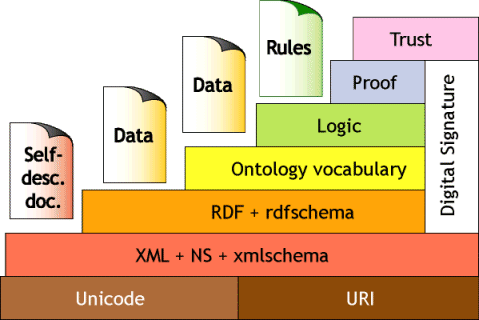
\includegraphics[scale=0.5]{layercake}
            \end{center}
            \begin{flushright}
                \texttt{[w3.org]}
            \end{flushright}
            This talk focuses on layers 3 and 4 
        \end{frame}

       \begin{frame}
            \frametitle{History}

            Important points in the history of the semantic web:
            \pause
            \vskip 0.7cm

            \begin{itemize}
                \item Some initial work during 1997-1998
                \pause
                \item In 1999
                    \pause
                    \begin{itemize}
                        \item February: First recommendation, RDF model and syntax
                        \pause
                        \item March: rdfschema proposal
                    \end{itemize}
                \pause
                \item February 2004: A suite of RDF and OWL recommendations, rdfschema recommendation
                \pause
                \item Most widely used since for RSS-feeds (but not known for that\ldots)
                \pause
                \item My first contact with it: 2003
            \end{itemize}
        \end{frame}




    \section{RDF}

        \begin{frame}
            \frametitle{Basic concepts}

            \large
            \textit{``Everything should be representable, so one needs a common model with great generality''}
            \vskip 0.3cm
            \textit{``Two basic elements:\\
            Assertions\\
            Quotations (statements about assertions)''}
            \vskip 0.3cm
            \begin{flushright}
                \texttt{[http://www.w3.org/DesignIssues/Semantic.html]}
            \end{flushright}
        \end{frame}


        \begin{frame}
            \frametitle{RDF model}

            This leads to a very simplistic model, to RDF:
            \vskip 0.7cm
            \pause

            \begin{itemize}
                \item Information is represented as a \textit{triple}, as a statement
                \pause
                \item Every triple consists of three elements:
                \pause
                \begin{itemize}
                    \item \textbf{Subject}
                    \pause
                    \item \textbf{Predicate}
                    \pause
                    \item \textbf{Object}
                    \pause
               \end{itemize}
               \item Subjects and predicates are given as URIs
               \pause
               \item Objects can either be other URIs or literal data
               \pause
               \item RDF data is represented by directed graphs 
           \end{itemize}
        \end{frame}

        \begin{frame}
            \frametitle{Example\ldots}
            \textit{``Mary has a lamb.''\\
            \pause
            \textit{``Mary is 14.''}\\
            \pause
            ``Big bad wolf wants this lamb.''\\
            \pause
            ``Big bad wolf engages the seven dwarfs.''\\
            \pause
            ``The seven dwarfs must catch the lamb.''\\}
            \pause
            \ldots and of course\ldots\\
            \pause
            \textit{``the lamb is an animal!''}
            \pause
        \end{frame}

        \begin{frame}
            \frametitle{Example - graph}

            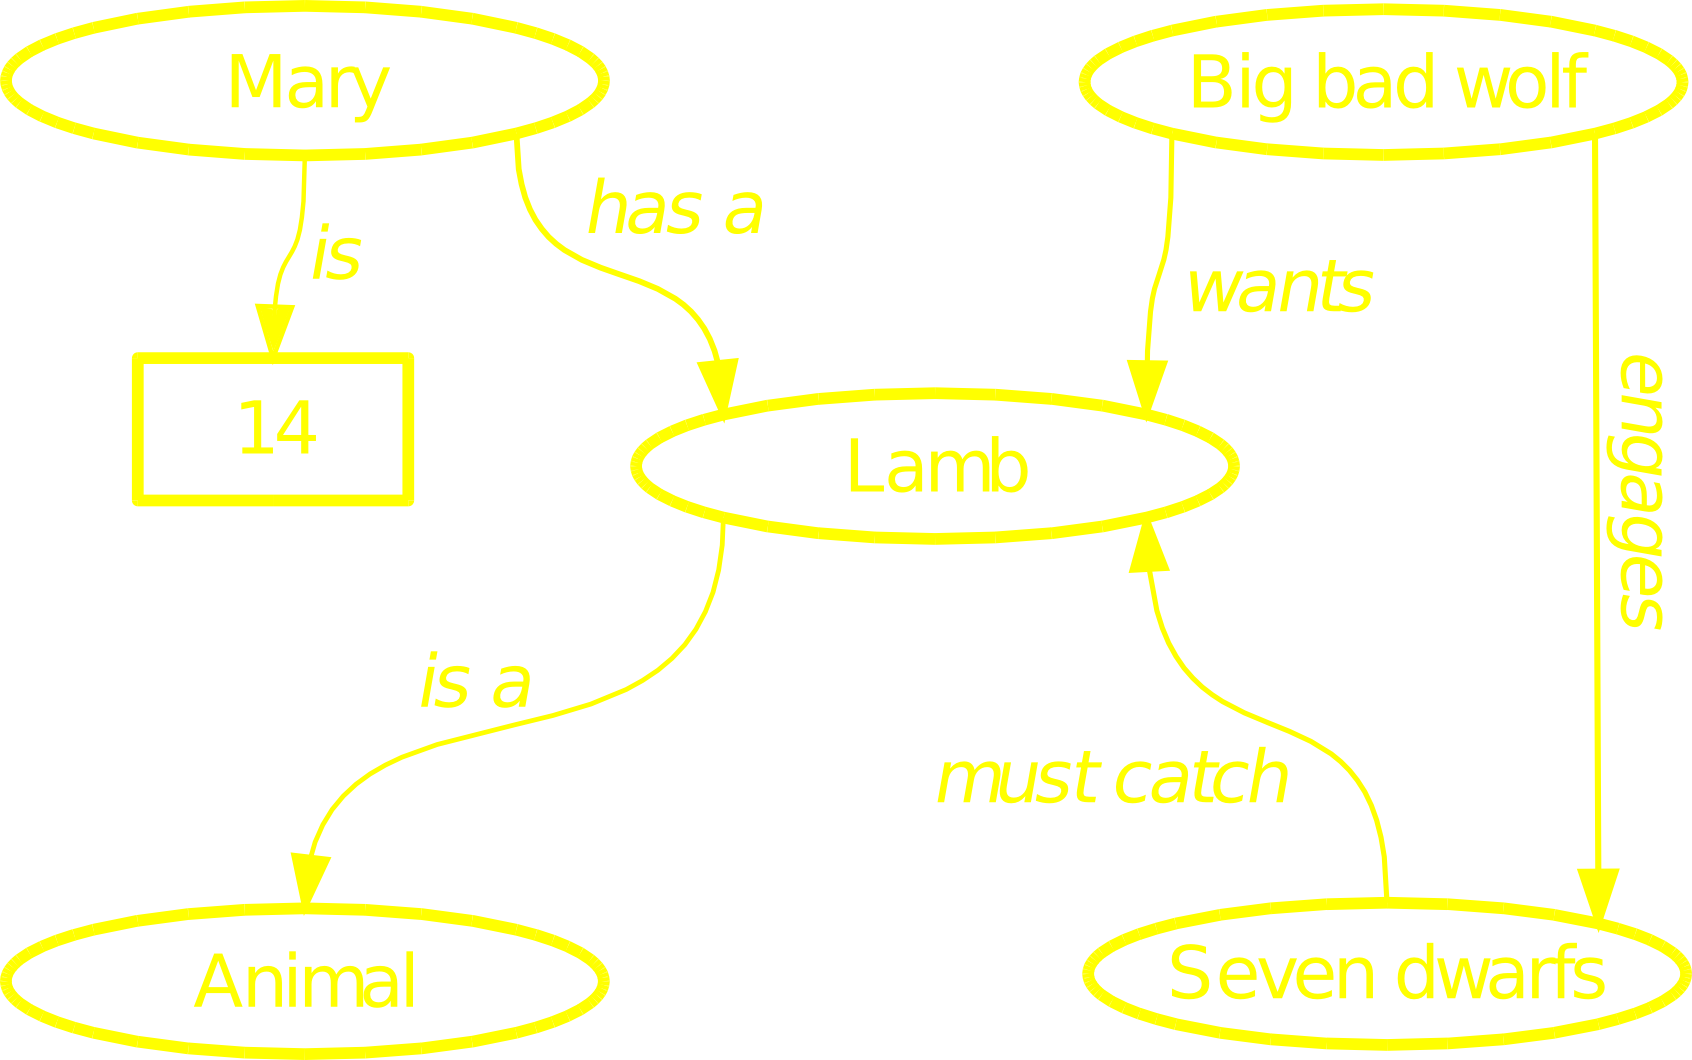
\includegraphics[scale=0.7]{graph}
        \end{frame}

        \begin{frame}
            \frametitle{Serialisation}
    
            And for the machines...
            \vskip 0.7cm
            \begin{itemize}
                \item \textbf{Notation 3 (N3)} - first form, quite complex
                \pause
                \item \textbf{N-Triples} - subset of N3, possible recommendation
                \pause
                \item \textbf{Turtle} - extension of N3
                \pause
                \item \textbf{XML}
                \pause
           \end{itemize}
           \vskip 0.7cm
       \end{frame}

       \begin{frame}
           \frametitle{Example - turtle serialisation 1}
           \footnotesize
           \texttt{\ding{229} <http://example.org/Mary>    <http://example.org/has>    <http://example.org/Lamb>  .\\
           \ding{229} <http://example.org/Mary>    <http://example.org/is>     ``14''  .\\
           \ding{229} <http://example.org/BigBadWolf>    <http://example.org/wants>   <http://example.org/Lamb>  .\\
           \ding{229} <http://example.org/BigBadWolf>    <http://example.org/engages>    <http://example.org/SevenDwarfs>  .\\
           \ding{229} <http://example.org/SevenDwarfs>    <http://example.org/muststeal>    <http://example.org/Lamb>  .\\
           \ding{229} <http://example.org/Lamb>    <http://example.org/isa>    <http://example.org/Animal>  .}
           \normalsize
           \vskip 0.7cm
           \textit{Note: lines are split up due to space. Each line starts with \ding{229}}
       \end{frame}

       \begin{frame}
           \frametitle{Example - turtle serialisation 2}
           Of course this isn't very handy, so here is a more cleaned up version:
           \footnotesize
           \vskip 0.7cm
           \texttt{\ding{229} @prefix ex: <http://example.org> . \\
           \ding{229} ex:Mary          ex:has          ex:Lamb ; \\
           \ding{229}                  ex:is           ``14''  . \\
           \ding{229} ex:BigBadWolf    ex:wants        ex:Lamb ; \\
           \ding{229}                  ex:engages      ex:SevenDwarfs  . \\           
           \ding{229} ex:SevenDwarfs   ex:muststeal    ex:Lamb . \\
           \ding{229} ex:Lamb          ex:isa          ex:Animal}
           \normalsize
           \vskip 0.7cm
           \textit{Note: Turtle provides also other shortcuts not shown here}
       \end{frame}

       \begin{frame}
           \frametitle{Example - XML serialisation}
           \vskip 0.8cm
           Example: XML-Serialisation\ldots
       \end{frame}
 
       \begin{frame}
           \frametitle{RDF - additional features}
           \begin{itemize}
               \item Typed literals: literals are identified by an URI. Example: XMLSchema-datatypes
               \pause
               \item Localisation of literals (language specific literals)
               \pause
               \item Empty nodes for complex relationships
               \pause
               \item Containers, lists, collections
               \pause
           \end{itemize}
       \end{frame}


    \section{rdfschema}

       \begin{frame}
           \frametitle{rdfschema - simple ontologies}

           rdfschema can be used to describe simple \textbf{ontologies}.
           \vskip 0.7cm
           \pause
           \textbf{Ontology???}
           \vskip 0.3cm
           \pause
           \textbf{Taxonomy???}
       \end{frame}

       \begin{frame}
           \frametitle{rdfschema - simple ontologies}

           \begin{itemize}
               \item Basic mechanisms for structuring RDF data
               \pause
               \item often already sufficient for simple ontologies
               \pause
               \item Example: Dublin Core
            \end{itemize}
       \end{frame}

       \begin{frame}
           \frametitle{Features of rdfschema}

           The most important constructs given by rdfschema are:
           \vskip 0.7cm
           \pause
           \begin{itemize}
               \item \texttt{rdfs:Class, rdfs:subClassOf}
               \pause
               \item \texttt{rdfs:Property, rdfs:subPropertyOf, rdfs:range, rdfs:domain}
               \pause
               \item \texttt{rdfs:type}
               \pause
               \item \texttt{rdfs:Container} (used for lists, sequences etc.)
           \end{itemize}
       \end{frame}

       \begin{frame}
           \frametitle{rdfschema - examples}

           \texttt{ex:Person    rdfs:subClassOf     <http://genome.org/human>}
           \vskip 0.3cm
           \pause
           \texttt{ex:Mary    rdfs:type     ex:Person}
           \vskip 0.3cm
           \pause
           \texttt{ex:is    rdfs:subPropertyOf    <http://older.net/ageproperty>}
           \vskip 0.3cm
           \pause
           \texttt{ex:is    rdfs:range      ex:Person}
       \end{frame}

    \section{OWL}

       \begin{frame}
           \frametitle{OWL - introduction}

           \textbf{OWL} is the \textbf{W}eb \textbf{O}ntology \textbf{L}anguage
      \end{frame}

      \begin{frame}
           \frametitle{OWL - introduction}

           wait...
           
           wouldn't that be \textbf{WOL} and not \textbf{OWL}???
     \end{frame}

     \begin{frame}
           \frametitle{OWL - introduction}
           Yes, but according to W3C:
           \vskip 0.7cm
           \pause
           \begin{itemize}
               \item It's clear how to pronounce OWL\ldots
               \pause
               \item This acronym is great for making logos\ldots
               \pause
               \item OWLs are associated with wisdom\ldots
               \pause
               \item This makes up a great backstory\ldots
               \pause
           \end{itemize}
           \footnotesize  %TODO verbatim?
           \texttt{[http://lists.w3.org/Archives/Public/www-webont-wg/2001Dec/0169.html]} 
           \normalsize
           \pause
           \vskip 0.7cm
           A theory is also, that this comes from Winnie the Pooh, where the owl wasn't able to
           write her name correctly\ldots ;-)
     \end{frame}
 
       \begin{frame}
           \frametitle{OWL - variants}

           \textbf{OWL Full}\\
           \begin{itemize}
               \item Contains \textbf{OWL DL} and \textbf{OWL Lite}
               \item Very expressive
               \item Not decideable (that causes headaches to reasoners\ldots)
               \item Not fully supported by software
           \end{itemize}
           \pause
           \textbf{OWL DL}
           \begin{itemize}
               \item Contains \textbf{OWL Lite}
               \item Decideable
               \item Nearly fully software supported
           \end{itemize}
           \pause
           \textbf{OWL Lite}
           \begin{itemize}
               \item Decideable
               \item Fully software supported
               \item Less expressive
           \end{itemize}
       \end{frame}

       \begin{frame}
           \frametitle{OWL Lite - constructs}

           OWL Lite Provides lots of constructs like
           \vskip 0.7cm
           \begin{itemize}           
               \item (In-)Equality
               \item Property restrictions
               \item Cardinality restrictions
               \item Datatypes
               \item \textit{\ldots and others\ldots}
           \end{itemize}
           \vskip 0.7cm
           \textbf{Of course, all of this can be combined with rdfschema!}
       \end{frame}

      \begin{frame}
           \frametitle{OWL DL/Full - constructs}

           OWL DL and OWL Full introduce even more constructs:
           \vskip 0.7cm
           \begin{itemize}           
               \item oneOf
               \item disjointWith
               \item equivalentClass
               \item \textit{\ldots and others\ldots}
           \end{itemize}
           \vskip 0.7cm
           \textbf{Again - combineable with OWL Lite and rdfschema!}
       \end{frame}

       \begin{frame}
           \frametitle{Full example}

           Very simple example taken from wikipedia\ldots

       \end{frame}

    \section{And now...?}

       \begin{frame}
           \frametitle{And now...?}

            \large
            \textit{''It's very simple - \\
                you read the protocol \\
                and write the code.''}

           (Bill Joy)
      \end{frame}

       \begin{frame}
           \frametitle{APIs}

           For programmers\ldots \\
           \ldots Almost everything you need is already there\ldots
           \vskip 0.7cm
           \begin{itemize}           
               \item APIs
               \item Triplestores (RDF-Databases)
               \item Query-engines
               \item Reasoners
               \item \textit{\ldots and more!}
           \end{itemize}
           \vskip 0.7cm
           Check the linklist on the website of this speech for some hints\ldots
 
       \end{frame}

       \begin{frame}
           \frametitle{Linking open data}
            \begin{itemize}           
               \item The "web of data", "giant global graph"\ldots
               \item W3C initiative
               \item Consists of interlinked, openly accessible data
               \item 4.7 billion RDF triples, 142 milions of links
               \item \textbf{That's a huge amount of machine-readable knowledge already}
            \end{itemize}
            
       \end{frame}

       \begin{frame}
           \frametitle{Browse and query it!}
           
           Tabulator demo
       \end{frame}

       \begin{frame}
           \frametitle{Infering and Reasoning}

           Besides of these uses, also infering and reasoning are interesting applications of RDF.
           \vskip 0.3cm
           \pause
           You can understand those as making automatic assumptions about triples.
           As a (very simple) example, look at this:
           \vskip 0.3cm
           \pause
           \textit{When we know that all human beeings are born\ldots\\
           \ldots and we know that Tim Berners Lee is a human beeing\ldots\\
           \ldots we can automatically infer that Tim Berners Lee has been born!}
           \vskip 0.3cm
           \pause
           Reasoning and infering go into artificial intelligence. I won't go any
           further here too - but it's a very interesting field and you can - again
           find a lot of information and tools on the web!
       \end{frame}

    \section{Conclusion}

      \begin{frame}
           \frametitle{Questions}

           Are there any\ldots
           \vskip 0.7cm
           \huge
           \ldots Questions?!?
           \vskip 0.7cm
           \huge
           \ldots Answers?!?
           \normalsize


       \end{frame}

       \begin{frame}
           \frametitle{Thanks!}
           \vskip 0.7cm
           \huge
           Thanks a lot for your interest!
           \normalsize
           \vskip 0.7cm
           Check out 
           \vskip 0.5cm
           \texttt{http://impressionet.ch/semwebspeech3}
           \vskip 0.5cm
           to find all the information (soon)!
       \end{frame}

\end{document}

